% Point spreads for two runs of blah

\begin{figure}
\center

\begin{subfigure}[b]{0.8\textwidth}
	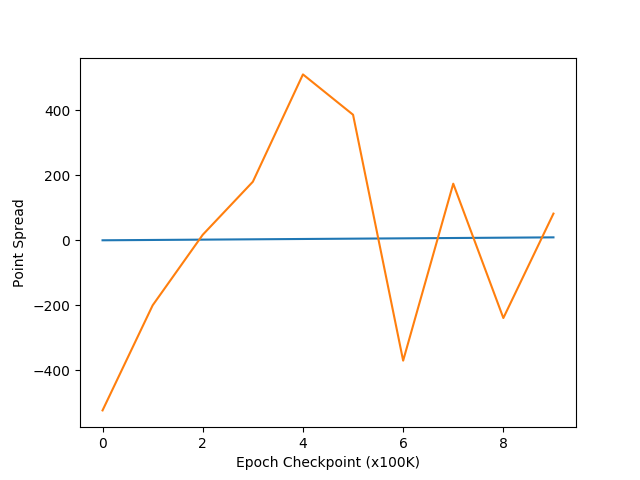
\includegraphics[width=\linewidth]{images/findings/round1/spread1.png}
	\label{fig_r1-spreads_a}
	\caption{}
\end{subfigure}

\begin{subfigure}[b]{0.8\textwidth}
	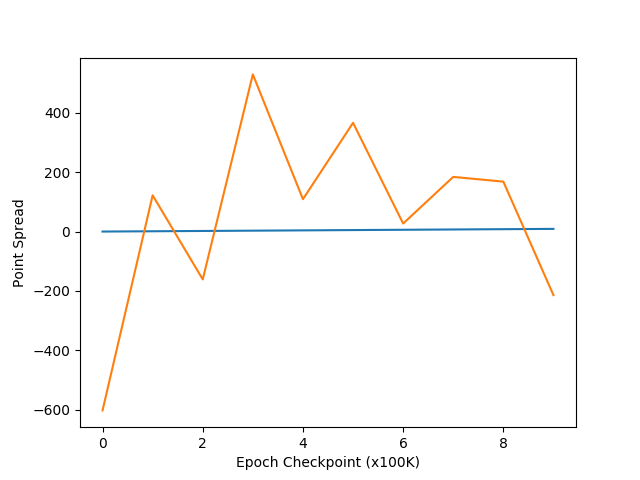
\includegraphics[width=\linewidth]{images/findings/round1/spread2.png}
	\label{fig_r1-spreads_b}
	\caption{}
\end{subfigure}

\caption{
	Point spreads across two 100-game tournaments pitting a winning
	agent against its checkpoints.
	Here, a positive point spread indicates that the fully-trained agent has
	accumulated more points than its opponent,
	an agent created from a checkpoint generated after the number of training
	game epochs indicated on the x-axis.
}
\label{fig_r1-spreads}
\end{figure}
